\documentclass[11pt]{article}
\usepackage{amsmath, amsfonts, amsthm}
\usepackage{amssymb}
\usepackage{xcolor}
\usepackage{tikz}
\usetikzlibrary{shapes,decorations,arrows,calc,arrows.meta,fit,positioning}
\tikzset{
    -Latex,auto,node distance =1 cm and 1 cm,semithick,
    state/.style ={ellipse, draw, minimum width = 0.7 cm},
    point/.style = {circle, draw, inner sep=0.04cm,fill,node contents={}},
    bidirected/.style={Latex-Latex,dashed},
    el/.style = {inner sep=2pt, align=left, sloped}
}
\usetikzlibrary{automata}

\begin{document}

	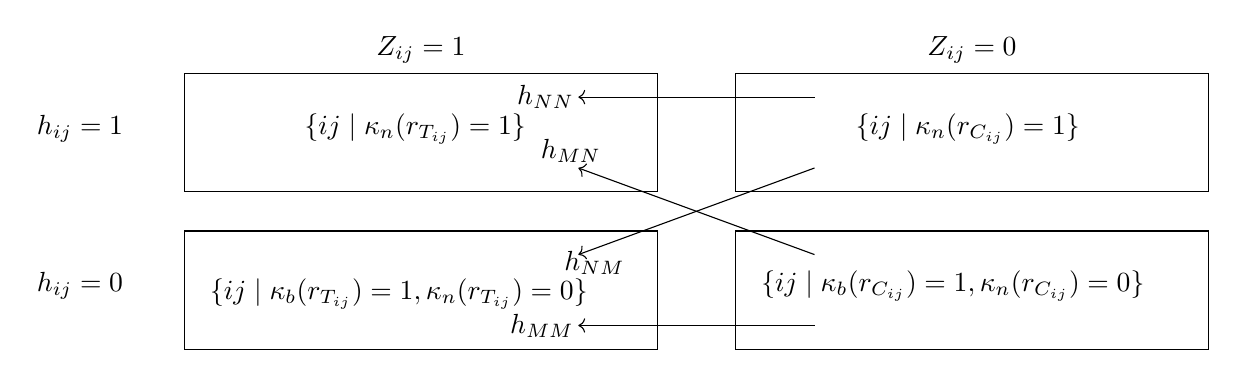
\begin{tikzpicture}
		\draw[draw=black] (10,5) rectangle ++(6,1.5);
		\draw[draw=black] (17,5) rectangle ++(6,1.5);
		\draw[draw=black] (10,3) rectangle ++(6,1.5);
		\draw[draw=black] (17,3) rectangle ++(6,1.5);
		\node[above] at (13,6.5) {$Z_{ij} = 1$};
		\node[above] at (20,6.5) {$Z_{ij} = 0$};
		\node[right] at (8,5.8) {$h_{ij} = 1$};
		\node[right] at (8,3.8) {$h_{ij} = 0$};
		\node[right] at (10.2,3.7) {$ \{ij\mid \kappa_b(r_{T_{ij}})= 1, \kappa_n(r_{T_{ij}})= 0 \} $ };
		\node[right] at (17.2,3.8) {$ \{ij\mid \kappa_b(r_{C_{ij}})= 1, \kappa_n(r_{C_{ij}})= 0 \} $ };
		\node[right] at (11.4,5.8) {$ \{ij\mid \kappa_n(r_{T_{ij}})= 1 \} $ };
		\node[right] at (18.4,5.8) {$ \{ij\mid \kappa_n(r_{C_{ij}})= 1 \} $ };
		\draw[->] (18,5.3) -- (15,4.2) node[pos=1.1,right] {$ h_{NM} $};
		\draw[->] (18,4.2) -- (15,5.3) node[pos=1.2,right] {$ h_{MN} $};
		\draw[->] (18,6.2) -- (15,6.2) node[pos=1.3,right] {$ h_{NN} $};
		\draw[->] (18,3.3) -- (15,3.3) node[pos=1.33,right] {$ h_{MM} $};
\end{tikzpicture}

\end{document}